\documentclass[conference,compsoc]{IEEEtran}
\usepackage{./macros}

\begin{document}
\vspace{3cm}
\title{CS5300 Assignment 3}
\author{Gautam Singh\\CS21BTECH11018}
\maketitle
\tableofcontents

\bigskip

\begin{abstract}
    This report analyzes C++ implementations of Filter and Bakery Locks. In
    particular, we compare the throughput, average and worst case critical
    section entry time for each implementation. The rest of the report is
    organized as follows. In \autoref{sec:prog-design}, we describe the
    low-level program design on which experiments are run. In
    \autoref{sec:results}, we compare the performance of both locks with varying
    parameters. Finally, we conclude the report in \autoref{sec:conclusion}.
\end{abstract}

\section{Program Design}
\label{sec:prog-design}

We give here an overview of the implementation details of the two programs, one
for the Filter Lock and one for the Bakery Lock.

\subsection{Threads and Runner Functions}
\label{subsec:threads-and-runners}
Threads are created using the C++ \texttt{std::thread} class. This makes it
convenient to pass thread IDs and references to other objects using
\texttt{std::ref} to the thread runner functions. In particular, we pass the
following arguments to the runner function.

\begin{enumerate}
    \item Thread ID from 0 to \(N - 1\), where \(N\) is the number of threads.
    This is because the \texttt{std::thread} class creates threads with IDs that
    may not be in this range, as they are only meant to be unique.
    \item Reference to the lock object.
    \item Logging output stream (a reference to a C++ \texttt{std::stringstream}
    object) to write timing information for further analysis and output.
\end{enumerate}

\subsection{Timing}
\label{subsec:timing}

The timestamps are reported using the \texttt{std::chrono} library. To prevent
zero values, we report times in nanoseconds, which is the smallest available
unit of time. However, results in the analysis are suitably scaled and reported
in milliseconds where needed.

\subsection{Random Number Generation}
\label{subsec:rng}

Random delays for simulating critical section and critical section request are
generated using exponential distributions with mean \(\lambda_1\) and
\(\lambda_2\). These distributions are instantiated as C++
\texttt{std::exponential\_distribution} objects. The randomness is generated
using a Mersenne Twister, instantiated using an \texttt{std::mt19937} object.
This random number generator is seeded using the current time since epoch.

\section{Results and Analysis}
\label{sec:results}

In this section, we analyze the performance of the locks on metrics such as
throughput and entry time when varying the total number of threads and the total
number of critical section requests made by each thread. This application was
run on an Intel i9-11900H processor.

\subsection{Throughput Analysis}
\label{subsec:throughput}

We define the throughput of our application to be the number of tasks completed
per unit time. In this case, accessing the critical section once is considered
as one task. Thus, the total throughput is \(\frac{NK}{T}\), where \(N\) is the
total number of threads, \(K\) is the number of critical section requests made
by each thread and \(T\) is the total time from creation to tear down of
threads.

\begin{figure}[!ht]
    \centering
    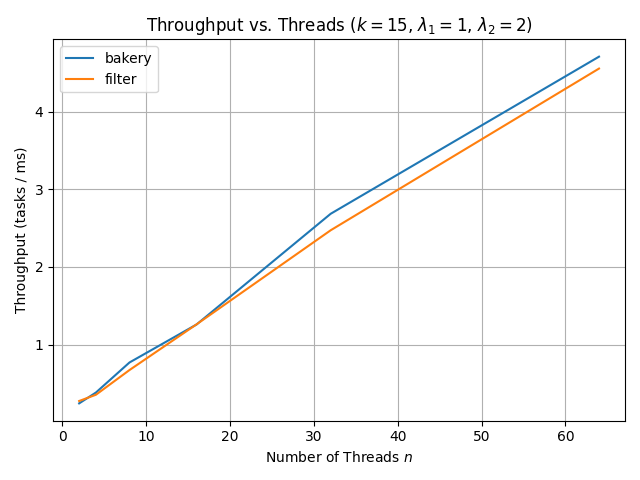
\includegraphics[width=\columnwidth]{images/exp1.png} 
    \caption{Throughput with varying number of threads.}
    \label{fig:exp1}
\end{figure}

\begin{figure}[!ht]
    \centering
    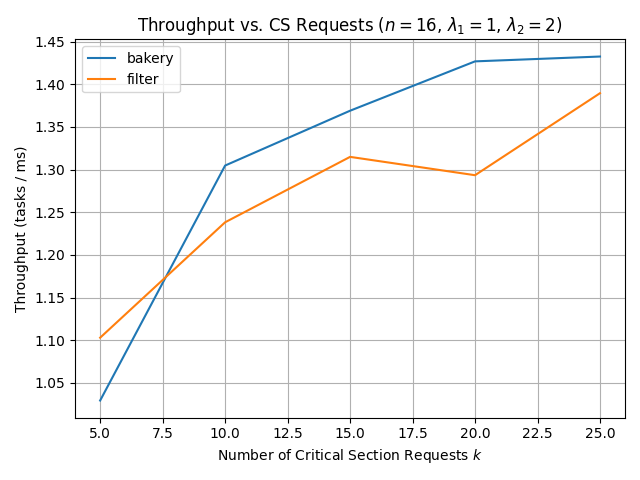
\includegraphics[width=\columnwidth]{images/exp2.png} 
    \caption{Throughput with varying number of critical section requests per thread.}
    \label{fig:exp2}
\end{figure}

\autoref{fig:exp1} depicts the variation of throughput with \(N\) and
\autoref{fig:exp2} depicts the variation of throughput with \(K\). We observe
the following.

\begin{enumerate}
    \item Throughput for both locks increases approximately linearly with \(N\).
    \item Throughput for both locks increases with \(K\).
    \item As \(K\) increases, the competition to enter the critical section
    levels off as the time in critical section tends to the mean \(\lambda_1\)
    of the exponential distribution, thus the rate of increase of throughput at
    a fixed \(N\) decreases for both locks.
    \item The bakery lock shows better throughput with increasing number of
    threads and critical section requests. This is because acquiring the filter
    lock involves more read/write operations as compared to the bakery lock. In
    other words, the lock method is much slower for the filter lock.
\end{enumerate}

\subsection{Entry Time Analysis}

The entry time is defined as the time taken to acquire the lock and enter the
critical section. We perform an average entry time analysis and a worst-case
entry time analysis for each lock implementation.

\begin{figure}[!ht]
    \centering
    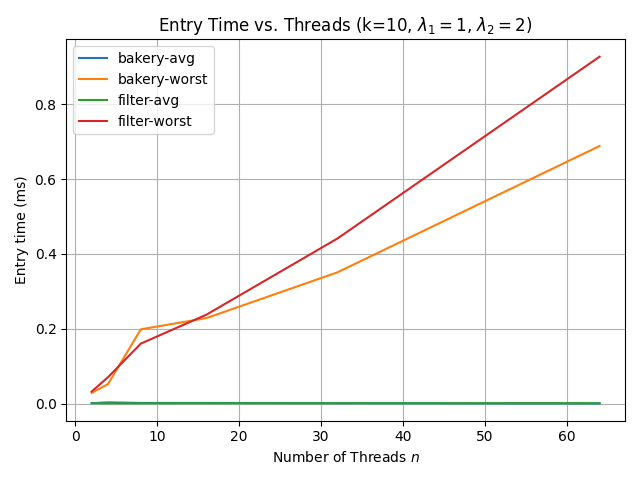
\includegraphics[width=\columnwidth]{images/exp3.png} 
    \caption{Entry time with varying number of threads.}
    \label{fig:exp3}
\end{figure}


\begin{figure}[!ht]
    \centering
    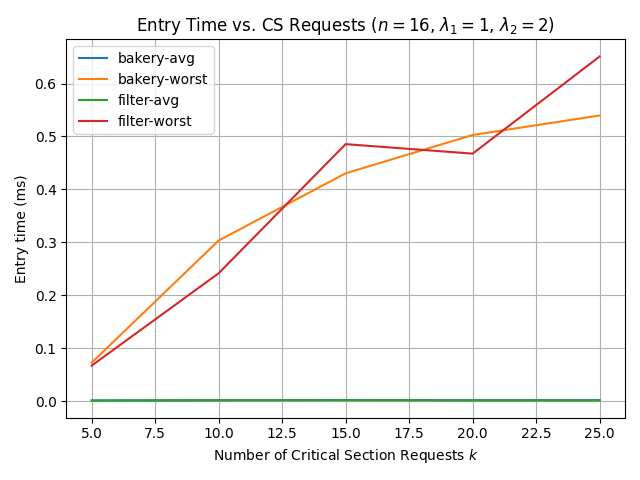
\includegraphics[width=\columnwidth]{images/exp4.png} 
    \caption{Entry time with varying number of critical section requests per thread.}
    \label{fig:exp4}
\end{figure}

\autoref{fig:exp3} depicts the variation of average and worst-case entry time
with \(N\) and \autoref{fig:exp4} depicts the variation of average and
worst-case entry time with \(K\) for both locks. We observe the following.

\begin{enumerate}
    \item The average entry time for both locks is comparable across various
    values of \(N\) and \(K\). Thus, on an average, there is no noticable
    difference in the entry time of a thread.
    \item The worst-case entry time of each lock has an approximately linear
    relation with \(N\), since there is increased competition to acquire the
    lock and enter the critical section.
    \item The worst-case entry time increases with \(K\) as well, since threads
    are making more requests to enter the critical section.
    \item The bakery lock has lower worst-case entry time than the filter lock,
    which could be due to the slow lock method in the filter lock and more
    chances of a thread waiting in trying to acquire the filter lock.
\end{enumerate}

\section{Conclusion}
\label{sec:conclusion}

From the analysis, we conclude that the bakery lock demonstrates marginally
better throughput and entry time performance than the filter lock, mainly due to
the slow lock method in the filter lock.

\end{document}